\documentclass{beamer}

\pdfmapfile{+sansmathaccent.map}


\mode<presentation>
{
  \usetheme{Warsaw} % or try Darmstadt, Madrid, Warsaw, Rochester, CambridgeUS, ...
  \usecolortheme{seahorse} % or try seahorse, beaver, crane, wolverine, ...
  \usefonttheme{serif}  % or try serif, structurebold, ...
  \setbeamertemplate{navigation symbols}{}
  \setbeamertemplate{caption}[numbered]
} 


%%%%%%%%%%%%%%%%%%%%%%%%%%%%
% itemize settings

\definecolor{mypink}{RGB}{255, 30, 80}
\definecolor{mydarkblue}{RGB}{60, 160, 255}
\definecolor{myblackblue}{RGB}{40, 40, 120}
\definecolor{myblue}{RGB}{240, 240, 255}
\definecolor{mygreen}{RGB}{0, 200, 0}
\definecolor{mygreen2}{RGB}{205, 255, 200}
\definecolor{mygray}{gray}{0.8}
% \definecolor{mydarkgray}{gray}{0.4}
\definecolor{mydarkgray}{RGB}{80, 80, 160}

\setbeamertemplate{itemize items}[default]

\setbeamertemplate{itemize item}{\color{myblackblue}$\blacksquare$}
\setbeamertemplate{itemize subitem}{\color{mydarkblue}$\blacktriangleright$}
\setbeamertemplate{itemize subsubitem}{\color{mygray}$\blacksquare$}

\setbeamercolor{palette quaternary}{fg=white,bg=mydarkgray}
\setbeamercolor{titlelike}{parent=palette quaternary}

\setbeamercolor{palette quaternary2}{fg=black,bg=myblue}
\setbeamercolor{frametitle}{parent=palette quaternary2}

\setbeamerfont{frametitle}{size=\Large,series=\scshape}
\setbeamerfont{framesubtitle}{size=\normalsize,series=\upshape}





%%%%%%%%%%%%%%%%%%%%%%%%%%%%
% block settings

\setbeamercolor{block title}{bg=red!30,fg=black}

\setbeamercolor*{block title example}{bg=mygreen!40!white,fg=black}

\setbeamercolor*{block body example}{fg= black, bg= mygreen2}


%%%%%%%%%%%%%%%%%%%%%%%%%%%%
% URL settings
\hypersetup{
    colorlinks=true,
    linkcolor=blue,
    filecolor=blue,      
    urlcolor=blue,
}

%%%%%%%%%%%%%%%%%%%%%%%%%%

\renewcommand{\familydefault}{\rmdefault}

\usepackage{amsmath}
\usepackage{mathtools}

\usepackage{subcaption}

\usepackage{qrcode}

\DeclareMathOperator*{\argmin}{arg\,min}
\newcommand{\bo}[1] {\mathbf{#1}}

\newcommand{\dx}[1] {\dot{\mathbf{#1}}}
\newcommand{\ma}[4] {\begin{bmatrix}
    #1 & #2 \\ #3 & #4
    \end{bmatrix}}
\newcommand{\myvec}[2] {\begin{bmatrix}
    #1 \\ #2
    \end{bmatrix}}
\newcommand{\myvecT}[2] {\begin{bmatrix}
    #1 & #2
    \end{bmatrix}}
    
    

\newcommand{\mydate}{Spring 2022}
\newcommand{\mygit}{\textcolor{blue}{\href{https://github.com/SergeiSa/Control-Theory-Slides-Spring-2022}{github.com/SergeiSa/Control-Theory-Slides-Spring-2022}}}


\newcommand{\bref}[2] {\textcolor{blue}{\href{#1}{#2}}}




%%%%%%%%%%%%%%%%%%%%%%%%%%%%
% code settings

\usepackage{listings}
\usepackage{color}
% \definecolor{mygreen}{rgb}{0,0.6,0}
% \definecolor{mygray}{rgb}{0.5,0.5,0.5}
\definecolor{mymauve}{rgb}{0.58,0,0.82}
\lstset{ 
  backgroundcolor=\color{white},   % choose the background color; you must add \usepackage{color} or \usepackage{xcolor}; should come as last argument
  basicstyle=\footnotesize,        % the size of the fonts that are used for the code
  breakatwhitespace=false,         % sets if automatic breaks should only happen at whitespace
  breaklines=true,                 % sets automatic line breaking
  captionpos=b,                    % sets the caption-position to bottom
  commentstyle=\color{mygreen},    % comment style
  deletekeywords={...},            % if you want to delete keywords from the given language
  escapeinside={\%*}{*)},          % if you want to add LaTeX within your code
  extendedchars=true,              % lets you use non-ASCII characters; for 8-bits encodings only, does not work with UTF-8
  firstnumber=0000,                % start line enumeration with line 0000
  frame=single,	                   % adds a frame around the code
  keepspaces=true,                 % keeps spaces in text, useful for keeping indentation of code (possibly needs columns=flexible)
  keywordstyle=\color{blue},       % keyword style
  language=Octave,                 % the language of the code
  morekeywords={*,...},            % if you want to add more keywords to the set
  numbers=left,                    % where to put the line-numbers; possible values are (none, left, right)
  numbersep=5pt,                   % how far the line-numbers are from the code
  numberstyle=\tiny\color{mygray}, % the style that is used for the line-numbers
  rulecolor=\color{black},         % if not set, the frame-color may be changed on line-breaks within not-black text (e.g. comments (green here))
  showspaces=false,                % show spaces everywhere adding particular underscores; it overrides 'showstringspaces'
  showstringspaces=false,          % underline spaces within strings only
  showtabs=false,                  % show tabs within strings adding particular underscores
  stepnumber=2,                    % the step between two line-numbers. If it's 1, each line will be numbered
  stringstyle=\color{mymauve},     % string literal style
  tabsize=2,	                   % sets default tabsize to 2 spaces
  title=\lstname                   % show the filename of files included with \lstinputlisting; also try caption instead of title
}


%%%%%%%%%%%%%%%%%%%%%%%%%%%%
% URL settings
\hypersetup{
    colorlinks=false,
    linkcolor=blue,
    filecolor=blue,      
    urlcolor=blue,
}

%%%%%%%%%%%%%%%%%%%%%%%%%%

%%%%%%%%%%%%%%%%%%%%%%%%%%%%
% tikz settings

\usepackage{tikz}
\tikzset{every picture/.style={line width=0.75pt}}


\title{Vector ODEs}
\subtitle{Math and modeling for high school}
\author{by Sergei Savin}
\centering
\date{Fall 2022}



\begin{document}
\maketitle


\begin{frame}{Scalar and vector equations}
	% \framesubtitle{Part 1}
	\begin{flushleft}
		
		Consider two differential equations:
		
		\begin{equation}
			\begin{cases}
				\dot x = -10x - 3t \\
				\dot y = -2y + t
			\end{cases}
		\end{equation}
	
		Introducing a vector variable $\bo{v} = [x, \ y]$ we can re-write the system as:
		
		\begin{equation}
		\dot{\bo{v}} = 
		\begin{bmatrix}
			-10 & 0 \\
			0 & -2
		\end{bmatrix}		
		\bo{v}
		+
		\begin{bmatrix}
			-3t \\
			t
		\end{bmatrix}
		\end{equation}		
		
		Notice that it is still two independent equations. But it doesn't have to be. Here is an example of a system of equations which are not interdependent:
		
		\begin{equation}
			\dot{\bo{v}} = 
			\begin{bmatrix}
				-10 & \textcolor{red}{2} \\
				0 &  -2
			\end{bmatrix}		
			\bo{v}
			+
			\begin{bmatrix}
				-3t \\
				t
			\end{bmatrix}
		\end{equation}		
		
	\end{flushleft}
\end{frame}




\begin{frame}{Vector ODEs}
	% \framesubtitle{Part 1}
	\begin{flushleft}
		
		In general, consider equation
		
		\begin{equation}
			\dot{\bo{v}} = 
			\bo{A}\bo{v}
			+
			\bo{c}
		\end{equation}		
		
		As before, we can discuss how the derivative of a variable in a ratio between the increase in its value and the time interval over which the increase has taken place:
		
		\begin{equation}
	\dot{\bo{v}} \approx
	\frac{\bo{v}(t + \Delta t) - \bo{v}(t)}{\Delta t}
		\end{equation}				
		
		So, we can make it into an \emph{integration scheme}:
		
		\begin{equation}
			\bo{v}(t + \Delta t) = \bo{v}(t) + (\bo{A}\bo{v}(t) + \bo{c}) \Delta t
		\end{equation}			
		
	\end{flushleft}
\end{frame}



\begin{frame}{Satellite problem}
	% \framesubtitle{Part 1}
	\begin{flushleft}
		
		When do system of ODEs become important?
		
		\bigskip
		
		Consider a problem: given a satellite orbiting Earth at the velocity $\bo{v}$, at the height $h$. Find its orbit.
		
		\bigskip
		
		Sounds quite intimidating, doesn't it?
		
	\end{flushleft}
\end{frame}




\begin{frame}{Satellite problem}
\framesubtitle{Newton's law}
	\begin{flushleft}
		
		First, let us remember the Newton's law:
		
		\begin{equation}
			m \dot{\bo{v}} = \bo{f}
		\end{equation}
		
		where $m$ is the mass of the satellite, $\bo{v}$ is its velocity and $\bo{f}$ is the sum of all external forces acting on the satellite.
		
		\bigskip
		
		Second, we assume that the only external force acting on the satellite is gravitational force.
		
	\end{flushleft}
\end{frame}



\begin{frame}{Satellite problem}
\framesubtitle{Gravity model}
	\begin{flushleft}
		
		For us it will be insufficient to assume that the gravity force is given by $mg$ directed towards the center of the Earth. Instead, we want to use a more precise model of gravitational force:
		
		\begin{equation}
			f = G \frac{m M}{h^2}
		\end{equation}
	
		where $f$ is the magnitude of the gravitational force, $m$ is the mass of the satellite, $M$ is the mass of the Earth and $h$ is the distance between the center of the Earth and the satellite.
	
		\bigskip
	
		Here are some of these constants:		
		\begin{itemize}
			\item $M = 5.972 \cdot 10^{24}$ kg
			\item $G = 6.673 \cdot 10^{-11}$ $\text{N m}^2/\text{kg}^2$
			\item radius of Earth is $6.371 \cdot 10^{6}$ m
		\end{itemize}
		
	\end{flushleft}
\end{frame}



\begin{frame}{Satellite problem}
 \framesubtitle{Position and gravity}
	\begin{flushleft}
		
		Let us assume that the position of the satellite relative to the center of the Earth, is given by the vector $\bo{r}$. How can we use this information to compute the magnitude of the gravity force?
		
		\bigskip
		
		Our strategy is to realize that $h = ||\bo{r}||$, and use it in the formula:
		
		\begin{equation}
			f = G \frac{m M}{||\bo{r}||^2}
		\end{equation}		 
		
	\end{flushleft}
\end{frame}



\begin{frame}{Satellite problem}
\framesubtitle{Direction of gravity}
	\begin{flushleft}
		
		But how do we give this force a direction? It always points towards Earth, so in the direction $-\bo{r}$. The gravity force should be pointing in the same direction. 
		\bigskip
		
		The way to ensure it, is to multiply the magnitude $f = G \frac{m M}{||\bo{r}||^2}$ by the direction unit vector $-\bo{r} /  ||\bo{r}||$:
		
		\begin{equation}
			f = -G \frac{m M}{||\bo{r}||^3} \bo{r}
		\end{equation}		 
		
	\end{flushleft}
\end{frame}


\begin{frame}{Satellite problem}
	\framesubtitle{Model}
	\begin{flushleft}
		
		Now we know the gravity force, and we can write the equations of motion for the satellite:
		
		\begin{equation}
			\begin{cases}
				\dot{\bo{r}} = \bo{v} \\
				m \dot{\bo{v}} = -G \frac{m M}{||\bo{r}||^3} \bo{r}
			\end{cases}
		\end{equation}
	
	Clearly we can divide the first equation by $m$, ridding us from this parameter - meaning the mass of the satellite does not play a role in this problem. This is true because we do not consider the effect of other forces than gravity, and we do not consider the effects the satellite has on the Earth.
		
	\end{flushleft}
\end{frame}



\begin{frame}[fragile]{Satellite problem}
	\framesubtitle{Code}
	\begin{flushleft}
		
		We can solve this system in MATLAB using the following code:
		
		\begin{lstlisting}[language=Matlab]
			G = 6.673 * 10^(-11);
			M = 5.972 * 10^24;
			r0 = randn(3, 1) * 7*10^6;
			v0 = randn(3, 1) * 1000;
			tspan = linspace(0, 20^4, 10^5);
			x0 = [r0; v0];
			odefun = @(t, x) [x(4:6); -G*M*x(1:3) / ... 
			((norm(x(1:3)))^3)];
			opts = odeset('Reltol',1e-13,'AbsTol',1e-14,'Stats','on');
			[t, x] = ode45(odefun,tspan,x0, opts);
			plot3(x(:, 1), x(:, 2), x(:, 3));
		\end{lstlisting}
		
		
		
	\end{flushleft}
\end{frame}



\begin{frame}{Satellite problem}
	\framesubtitle{Graph}
	\begin{flushleft}
		
		We plot the solution, and the result is shown below:
		
		% TODO: \usepackage{graphicx} required
		\begin{figure}
			\centering
			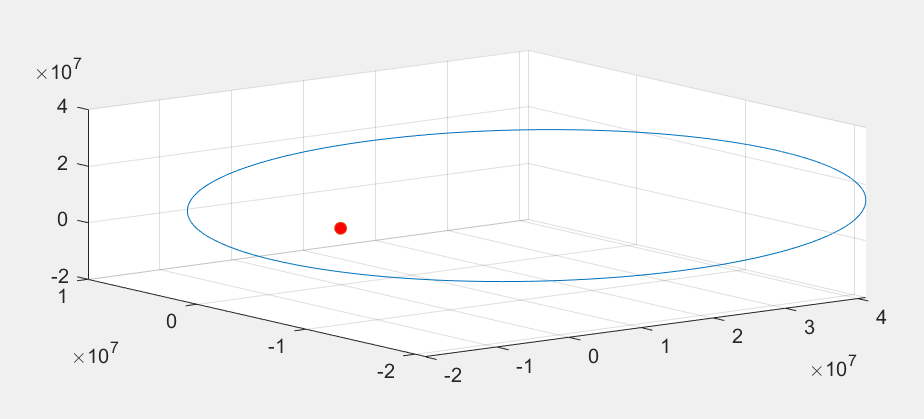
\includegraphics[width=0.9\linewidth]{Satellite}
			\caption{Orbit of a satellite, found by ode45; center of the Earth is given by a red dot}
			\label{fig:satellite}
		\end{figure}
		
		
	\end{flushleft}
\end{frame}




\begin{frame}{Thank you!}
\centerline{Lecture slides are available via Moodle.}
\bigskip
\centerline{You can help improve these slides at:}
\centerline{\mygit}
\bigskip
\centerline{Check Moodle for additional links, videos, textbook suggestions.}
\bigskip

\centerline{\textcolor{black}{\qrcode[height=1.6in]{https://github.com/SergeiSa/Extra-math-for-high-school}}}

\end{frame}

\end{document}
